\documentclass[12pt,a4paper]{article}
\usepackage[czech]{babel}
\usepackage[utf8]{inputenc}
\usepackage[colorlinks=true]{hyperref} % Aktivní odkazy
\usepackage{graphicx} %vkládání obrázků
\usepackage{authblk} %Formátování autorů
\usepackage{floatrow}
\usepackage{subfig}
\usepackage{subcaption}

\usepackage[backend=biber, style=iso-numeric, giveninits=true, maxbibnames=99]{biblatex} %spravuje interakci s literaturou, nastavuje ISO 690

\DeclareNameAlias{default}{last-first} %Formátování jmen v citacích
\makeatletter
\renewcommand\Authands{, } % Formátování autorů pro češtinu
\makeatother

\textwidth 15,92cm \textheight 24.62cm
\topmargin -2.2cm 
\oddsidemargin 0cm \evensidemargin 0cm

\pagestyle{empty}
\addbibresource{refs.bib}
\nocite{*} % Vytiskne celý .bib soubor bez nutnosti citovat

\title{Dálkové měření vzdálenosti pomocí laserového paprsku (LIDAR)}


\author[1]{Jakub Skalka}
\author[2]{Filip Landr}
\author[3]{Jaroslav Kraft}

\date{\small Garant: Ing. Kryštof Kadlec, KLFF FJFI\vspace{-2em}} % It is what it is. Je 16. 6. 9:00, je to šité horkou jehlou. \vspace je důležitý, jinak si budete krást místo pro příspěvek. Vždy musí být u posledního autora

\affil[1]{Gymnázium, České Budějovice, Jírovcova 8; skalkaj@jirovcovka.net}
\affil[2]{Gymnázium, Praha 5, Nad Kavalírkou 100/1; fi.landr@seznam.cz}
\affil[3]{Gymnázium, Příbram, Legionářů 402; kraft.jarda@gmail.com\vspace{-1em}} %Ditto, \vspace musí být u posledního autora

\begin{document}

\maketitle \thispagestyle{empty}

\begin{abstract} \noindent
    Náš příspěvek se zaměřuje na aplikaci technologie dálkového měření vzdálenosti - LIDAR (Light Detection And Ranging). Tato technika je založena na stanovení doby šíření laserového paprsku odraženého od snímaného objektu. \\Věnuje se také základům generace laserového záření a měření výstupních parametrů u Q-spínaného mikročipového laseru Nd:YAG.\end{abstract}


\section{Úvod}
Laser funguje na základě třech kvantových jevů. absorbce, spontánní emise a stimulovaná emise. Tyto jevy se dějí v aktivním prostředí všechny najednou a podle populace energetických hladin některé jevy převyšují jiné. Laser těhto jevů využívá, aby invertoval populace hladin iontů, tím se nabil a následně přes spontánní emisi přešel v emisi stimulovanou a fotony stimulované emise odrážel od zrcadel na koncích krystalu a umocňoval tak jejich počet (intenzitu zářeni) při každém průchodu resonátorem. A výstupovým částečně propustným zrcadlem odletí nějaké procento fotonů a ty tvoří laserové záření.
\\Q-spínání je jev, kdy se sníží jeden z kvantových jevů na minimum a to stimulovaná emise. Tímto způsobem lze ionty nabít na vyšší hladinu, než by bylo normálně možné a vytvořit velmi silný, krátký laserový impuls. Q-spínání je rozděleno na 2 typy, aktivní a pasivní. Aktivní spínání znamená, že mu musíme dodávat energii zvenčí (mechanicky ovládáme zrcadlo), pasivní q-spínání nastává chemicky, kdy je použit saturovatelný absorbér, ten mění svojí reflektivitu na základě přijmuté intensity záření, při dostatečné intensitě absorbér propouští veškeré záření.
\\mikročipový laser je speciální případ laseru, kdy jsou na aktivním prostředí zrcadla již nanesena a je snaza zmenšit laser do co nejmenšího objemu. pro mikročipový pasivně Q-spínaný laser to znamená, že aktivní prostředí je spojeno s absorbérem a na konce vzniklého válečku jsou nanesena zrcadla
\\LIDAR je metoda měření vzdálenosti pomocí odrazu laseru od překážky. Je využívaná například v topografii na utváření map a také map oceánů, dále se využívá například při těžení, plánování a mnohém dalším.
\\Je tato metoda však dostatečně přesná? Ubližuje nám záření z topografických letadel? Jaká je spolehlivost měření LiDARem a na čem je závislá?


\section{Popis našeho laseru}
Při našem pokusu jsme použili mikročipový pasivně Q-spínaný laser Nd:YAG/V:YAG, který vyzařoval ve spektrální oblasti $1,3$ $\mu$m, která je “eyesafe”, tedy bezpečná pro lidské oko. Náš laser měl tvar válce s průměrem $5$ mm a délka aktivního prostředí Nd:YAG byly $4$ mm a délka saturovatelného absorbéru V:YAG byla $0,7$ mm. počáteční transmise absorbéru byla $85$ \% a reflektivita výstupního zrcadla byla $90$ \% v již zmiňované spektrální oblasti. Koncentrace iontů Nd$^{3+}$ v YAG matrici bylo 1,1 \% Nd/Y. 
\\Náš pevnolátkový laser byl čerpán laserovou diodou na vlnové délce 808 nm, která už není oku bezpečná. Dioda byla použita v pulsním režimu s délkou impulsu 500 um a opakovací frekvencí 50Hz. Proud na diodě byl nastaven na 30 A a teplota byla 30 °C. Pro zefektivnění čerpání, byla dioda navedena optickým vláknem do fokusační optiky, tvořenou kolimátorem a fokusační čočkou.

\section{Měření výstupních parametrů laseru}
Pro správné určení laseru jsme potřebovali změřit střední výkon, délku a časový průběh impulsu, profil svazku, vyzařované spektrum, energii a špičkový výkon. Střední výkon jsme měřili pomocí powermetru THORLABS PM100USB a sondou THORLABS PM16-401. Délku a časový průběh laserového impulsu jsme měřili pomocí osciloskopu TEKTRONIX TDS 3052B a InGaAs fotodiodou (FGA10). Profil svazku jsme měřili křemíkovou CCD kamerou WinCamD. Vyzařované spektrum jsme naměřili InGaAs mřížkovým spektrometrem od Stellarnetu (DWARF-STAR). Energii a špičkový výkon jsme vypočítali podle vzorečků
$\frac{P_{str}}{f}$ a $\frac{E}{T}$.

\section{Postup měření}
Měření vzdálenosti metodou LiDAR probíhalo tak, že jsme si nastavili překážku pro laser v dané vzdálenosti a nechali jsme šířit laserový impuls dle schématu na obrázku, následně jsme pomocí osciloskopu detekovali časový průběh laserového impulsu který do fotodiody přišel přímo z děliče svazků a druhý impuls, který se odrazil od překážky. Pak jsme je porovnali na osciloskopu a ten nám udal časový rozdíl mezi impulsy a tím pádem nám dal potřebnou informaci pro výpočet vzdálenosti mezi rozdělovačem a zábranou. Vzdálenost jsme vypočítali pomocí tohoto vzorečku $\frac{c \cdot t}{2}$, díky kterému jsme dostali relativně přesné hodnoty s odchylkou měření do 60 cm, protože jeden puls laseru měl délku 60 cm, kdybychom pulzy dělali kratší, tak budeme mít vyšší přesnost, ale pro naše podmínky a zadání tato přesnost stačila.
\begin{figure}[h!]
    \centering
    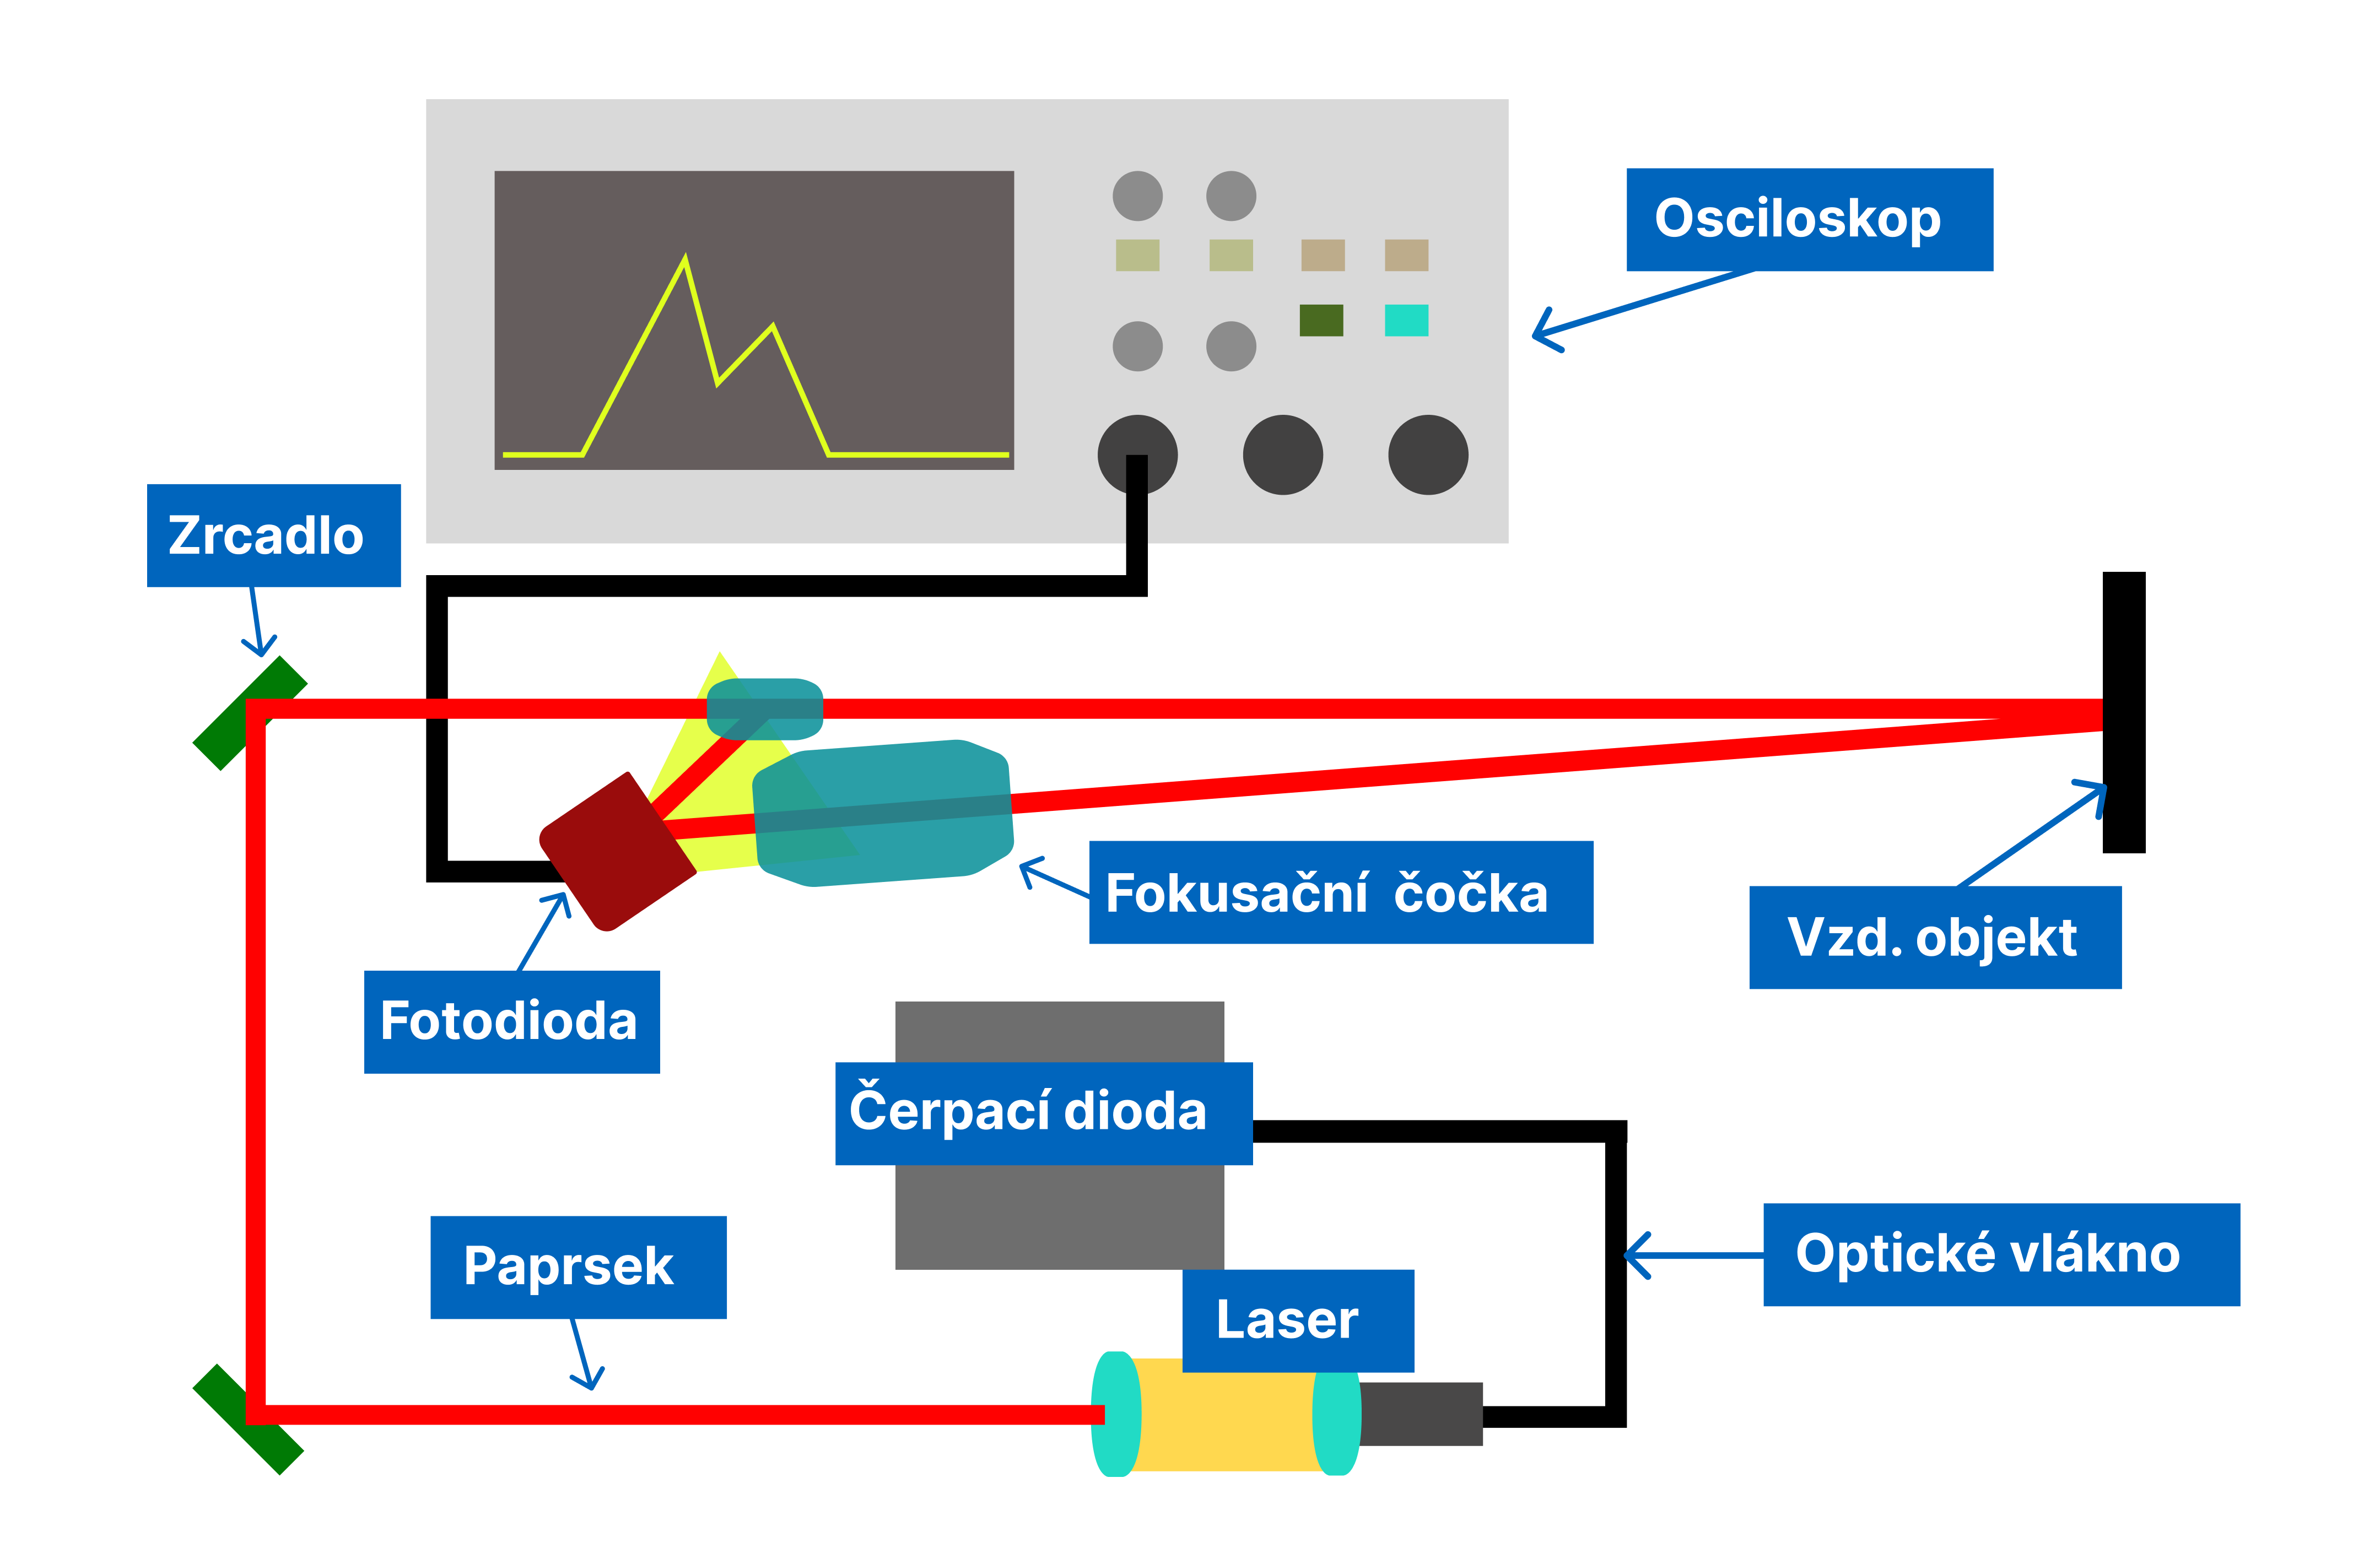
\includegraphics[width=0.5\textwidth]{Diagram měření.png}
    \caption{diagram měřící aparatury}
\end{figure}

\section{Výsledek měření}

\begin{center}
    \begin{tabular}{||c c c||} 
     \hline
      měření & d [cm] & t [ns] \\ [0.5ex] 
     \hline\hline
     zeď & 548 & 9.2 \\ 
     \hline
     1 metr & 100 & 6.6 \\
     \hline
     3 metry & 300 & 25.9 \\
     \hline
    \end{tabular}
    \end{center}
    
\begin{figure}[h!]
    \centering
    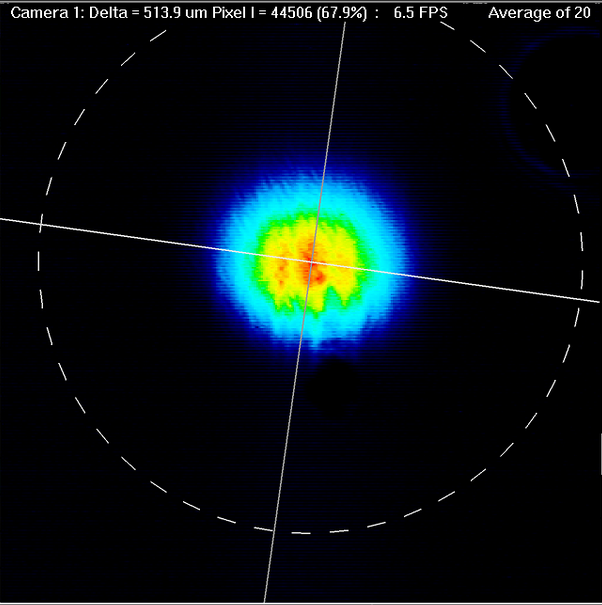
\includegraphics[width=0.5\textwidth]{profil.png}
    \caption{Profil svazku laseru}
\end{figure}

\begin{figure}[h!]
    \centering
    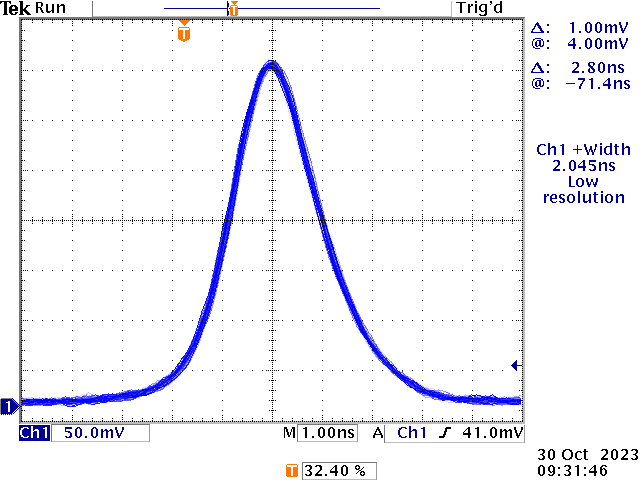
\includegraphics[width=0.5\textwidth]{prubeh_impulsu.png}
    \caption{Časový průběh laserového impulsu}
\end{figure}


\pagebreak
\section{Shrnutí}
Dle našich měření lze vyvodit, že LIDAR je přesnější na nižších délkách impulsu a tím pádem to je metoda, kde lze hodně zkoumat, ale je potřeba kvalitních laserových materiálů a lepších přístrojů, abychom dosáhly co nejkratších impulsů. Dále je potřeba dále vyvíjet metody detekce fotonů, jelikož u velmi malých pulzů letí malé množství elektronů a to nemusí být detekováno. Komerčně i armádně využívané lasery pro topografii metodou LIDAR jsou většinou pro oko bezpečné, kvůli jejich rychlé absorbci ve vodě, tudíž neprojdou až na sítnici a nepoškodí ji, avšak určitý typ laserů pro podvodní topografii je velmi pro oko zničující. Spolehlivost LIDARu je velmi závislá na počasí, jelikož se používají lasery absorbovatelné ve vodě, tak při vysoké vlhkosti se může paprsek absorbovat v atmosféře a nenaměřit vzdálenost žádnou. Naopak při intenzivním záření ze slunce je možné, že toto záření “přesvítí” používaný laser a výsledná data jsou také k ničemu.
Je to metoda, která je už v praxi docela hojně používaná, ale stále je možné ji zlepšovat.


\section*{Poděkování}
Chtěli bychom velice poděkovat Ing. Kryštofovi Kadlecovi za jeho pomoc a podporu při vytváření tohoto příspěvku.
Náš dík patří také FJFI za umožnění výzkumu v rámci projektu a KLFF za poskytnutí prostoru.
\printbibliography


\end{document}